\documentclass[12pt]{article}

\usepackage{geometry}
 \geometry{
 a4paper,
 left=25mm,
 right=20mm,
 top=20mm,
 }
 
\usepackage{hyperref}
\usepackage{exercise}
\usepackage{enumerate}
\usepackage{graphicx}
\usepackage{subfig}
\usepackage{listings}

\graphicspath{ {images/} }

\lstset{language=python, firstline=37, lastline=45, title={Listing 1: Data structures for cellular automaton}}

\begin{document}

\title{
Computational Geometry and Digital Images \\
\textbf{fork-recognition}\\
Project report
}

\author{Etienne Moutot, Ievgeniia Oshurko}
\date{April 6, 2016}
\maketitle


\section{Introduction}  

\section{Feature Engineering}

The extracted features capture the properties of shape: its topology and its geometry. In total, 38 features were developed:

\begin{itemize}
	\item Histogram of distance of the medial axis points from borders (\textbf{10 features} corresponding to 10 bins of histogram)
	\item Histogram of border curvature coefficients(\textbf{5 features} corresponding to 5 bins of histogram)
	\item Scaled area
	\item Solidity
	\item Extend
	\item Scaled major axis length
	\item Scaled minor axis length
	\item Histogram of medial axis straight lines length (\textbf{5 features} corresponding to 5 bins of histogram)
	\item Number of branches of medial axis skeleton
	\item Number of branched points of medial axis skeleton
	\item Scaled centroid displacement
	\item Asymmetry measures (\textbf{9 features} corresponding to horizontal and vertical flips, and rotation for 7 distinct angles)
\end{itemize} 

\subsection{Image preprocessing}
The images are pre-processed before we extract the features from them. There are two reasons for that:
\begin{itemize}
	\item We want to remove the noise from the image, because our features need to be robust to noise.
        \item We also want to remove the black holes that appears in some images.
        \item We want the shape to be white and the backgroud black (one of the rats is reversed).
\end{itemize}

For that we implemented 3 transfomations:
\begin{description}
	\item[Image padding]: The border of the image are just filled with a border of black pixels, in order to avoid problems when the shapes touch the border.
        \item[Shape filling]: The background is detected by the fact that it is the first connected component. Then it is fillend in black and the rest of the image (the main shape) is filled with white. With that we remove all the wholes in the image.
        \item[Smoothing]: The goal of this smoothing is to get rid of the noise at the border of the shape. We apply to the image a median filter, with as neighborhood a disk of a 7px diameter. After few tests, 7px seems to be a good compromise between smoothing and not loosing too much details. 
        
        \begin{figure}[h]
          \begin{center}
            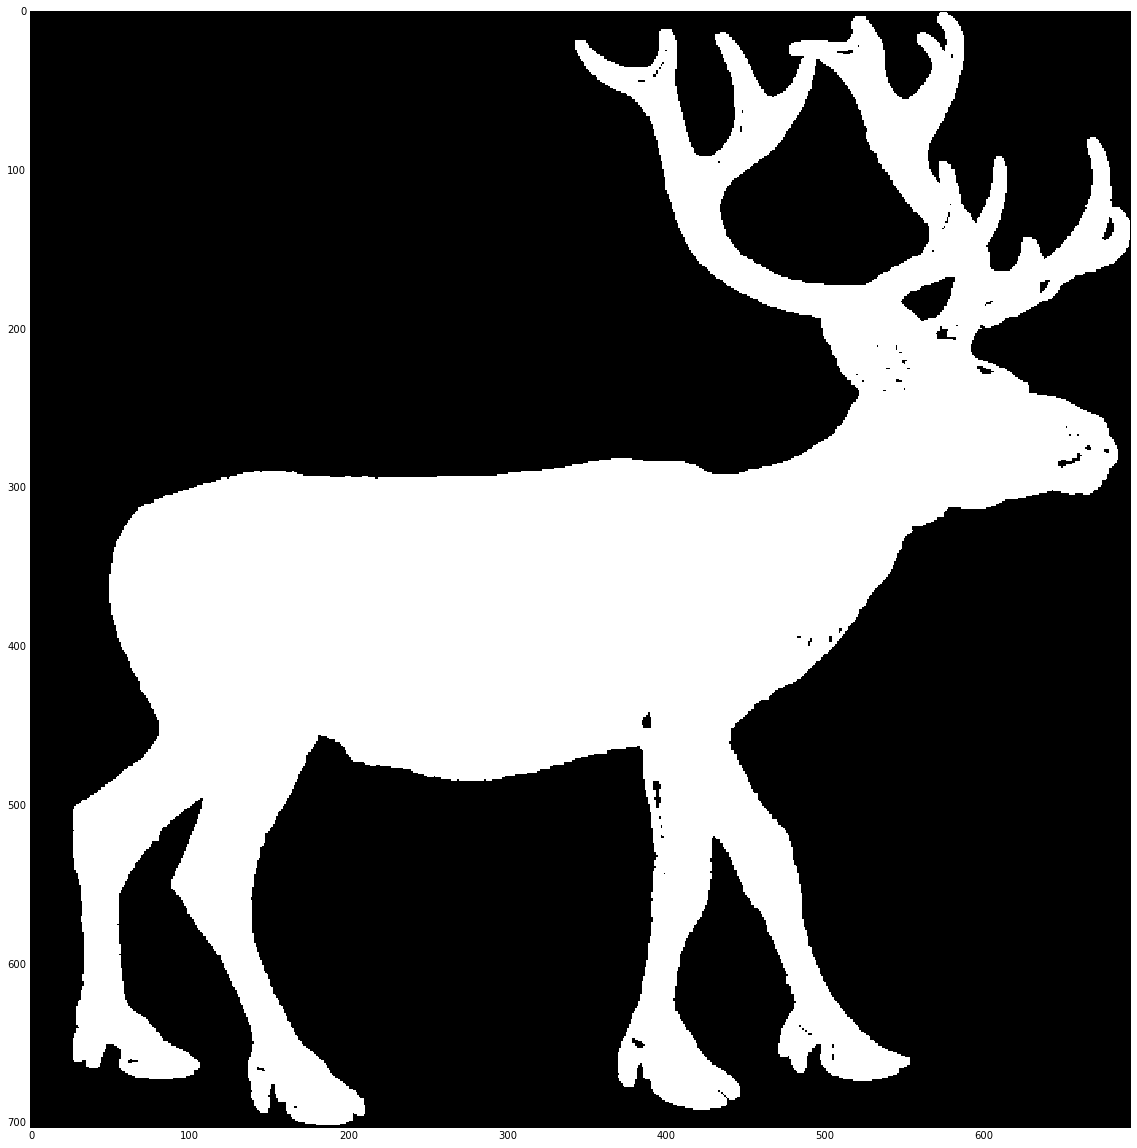
\includegraphics[scale=0.20]{deer_no_processing.png}
            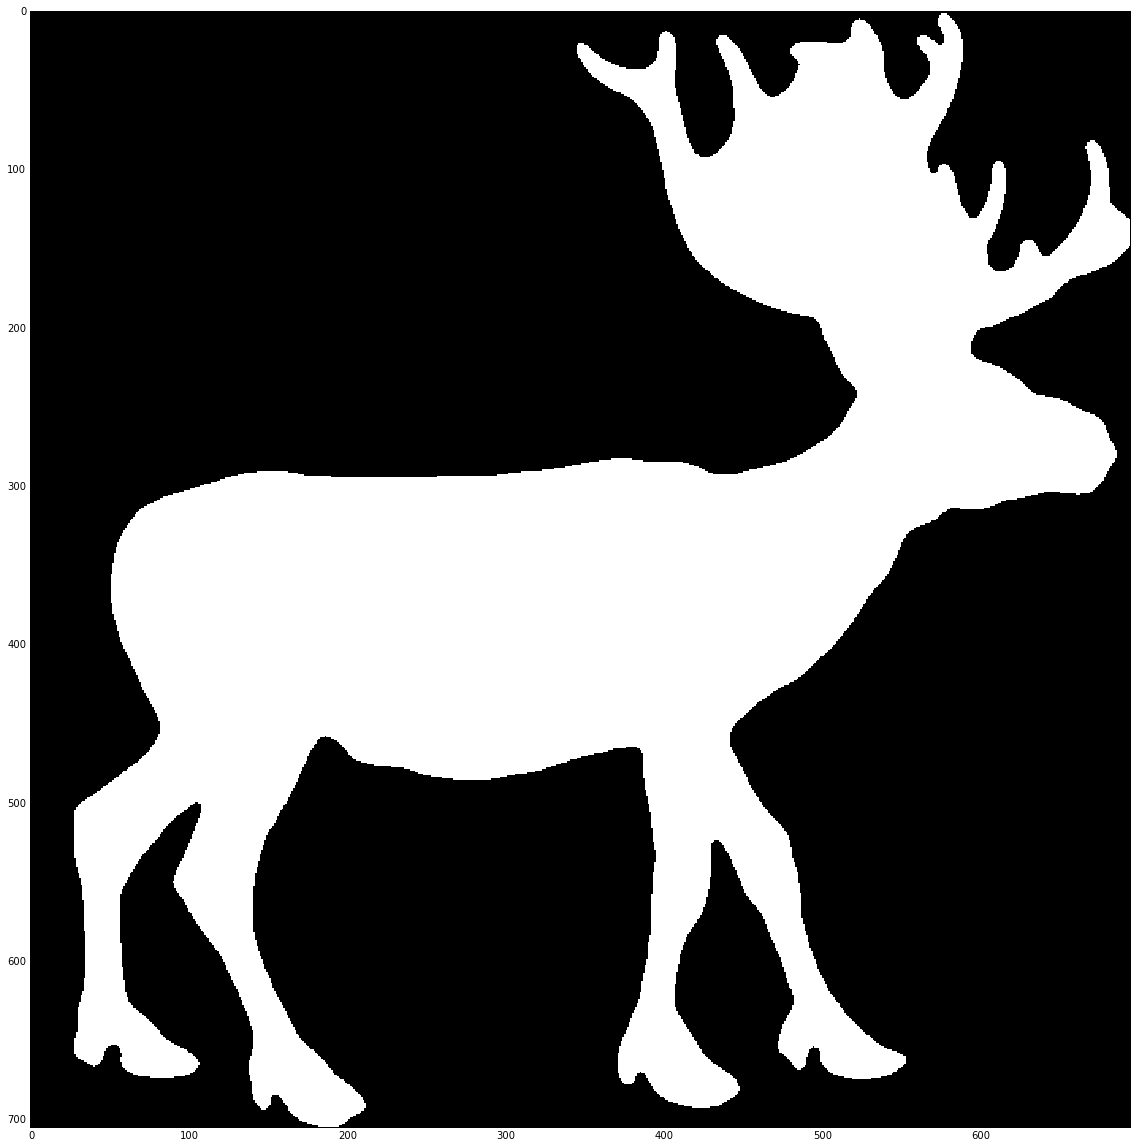
\includegraphics[scale=0.20]{deer_with_processing.png}
            \caption{Example without and with pre-processing}
          \end{center}
        \end{figure}
\end{description}

\subsection{Medial Axis}


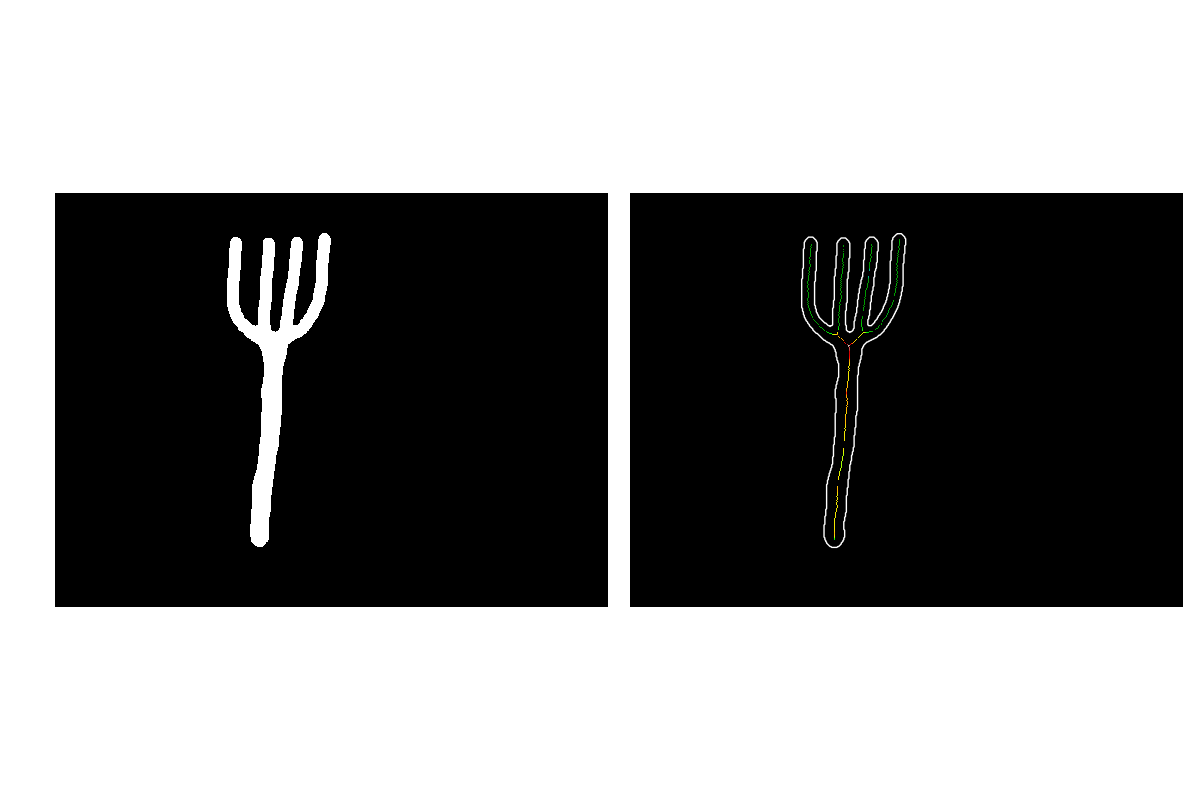
\includegraphics[scale=0.25]{fork_75.png}
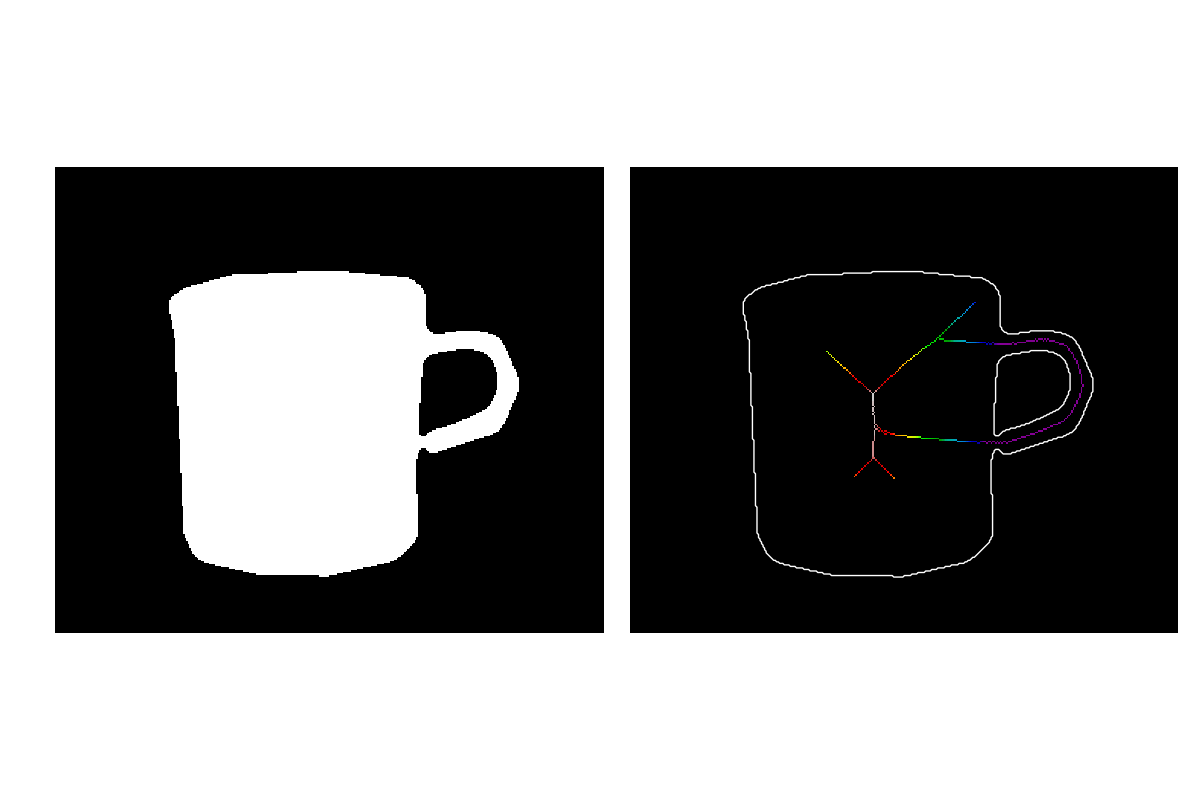
\includegraphics[scale=0.25]{cup_476.png}

\vspace{12px}

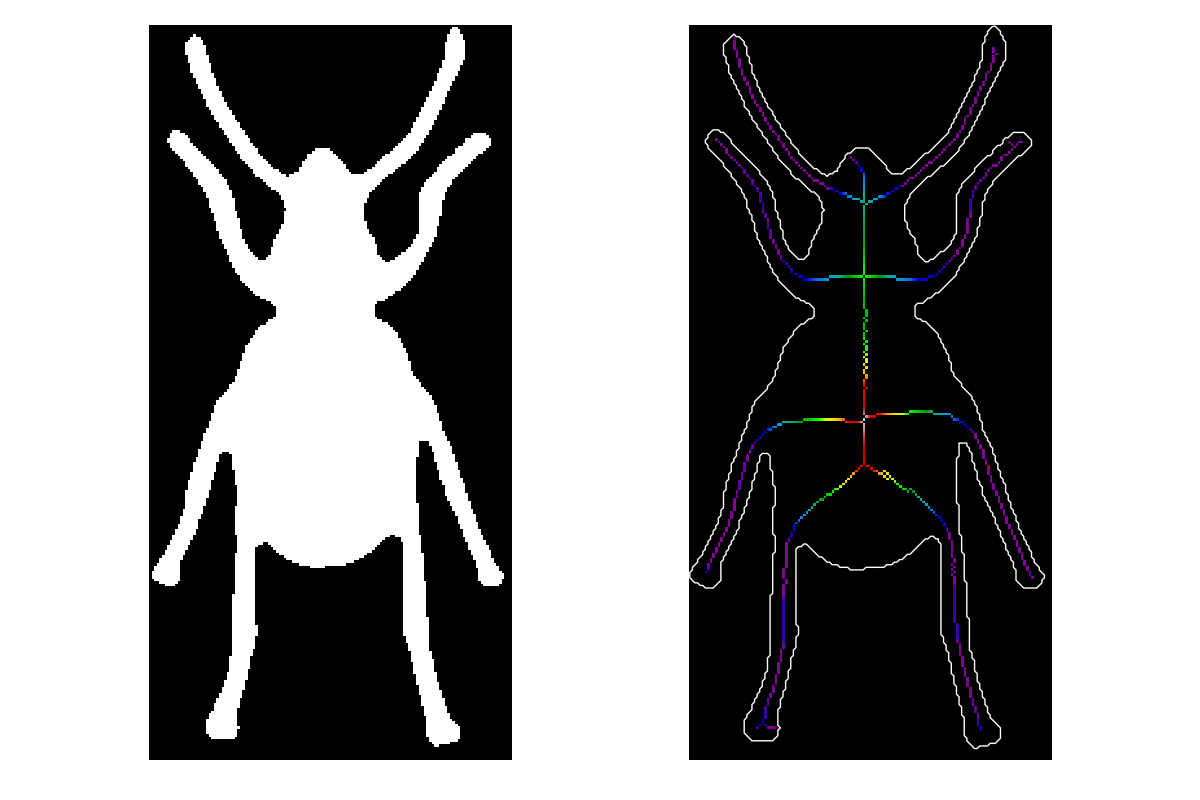
\includegraphics[scale=0.25]{beetle_281.png}
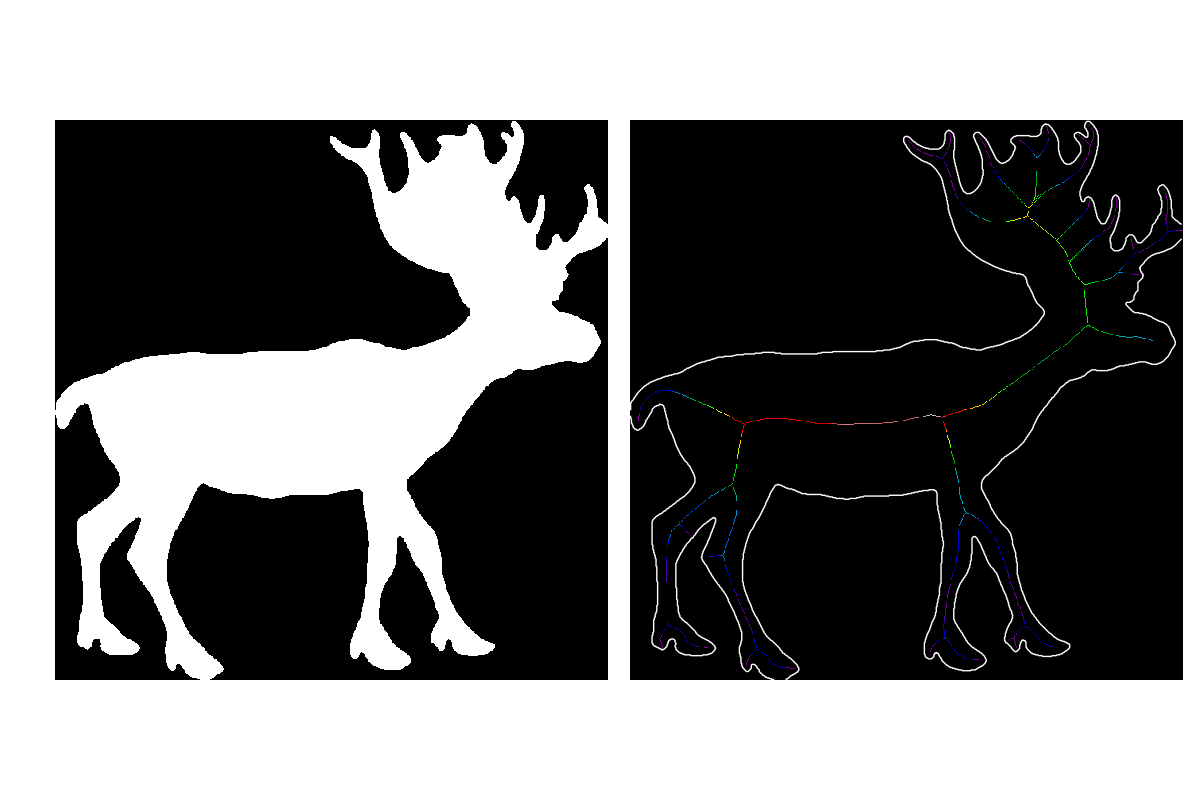
\includegraphics[scale=0.25]{deer_79.png}

\subsubsection{Histogram of distance of the medial axis points from borders}

Each point $p$ of medial axis skeleton has the value $d(p)$ of distance to the border  assigned to it, this distance may also be seen as the radius of the maximal incircle with a center in $p$, and, in general, characterises the local thinkness of the shape in this point. Histogram of the skeleton distaces was used as a feature for our shape description, and it gives us the information about the distribution of local thinkness of the given shape.

\subsubsection{Medial axis straight lines}

Python implementation (\texttt{skimage.transform.probabilistic\_hough\_line}) of \textit{Probabilistic Hough Transform} \cite{Kiryati} was used to detect straight lines in medial axis skeleton. In this method straight line is represented by the segment perpendicular to it, parametrised by a pair $(\rho, \theta)$, where $\rho$ is a length of segment, and $\theta$ is an angle. Hought transform consists of two steps: parameter's plane of $(\rho, \theta)$ is divided into discrete grid (by parameter histogram bins), and the array representing this grid contains number of pixels close to the respective line, after this the exhaustive search of the parameters with maximum frequency is performed. Each time you find a pixel close to a particular parametrised line you increment the corresponding value of an array, this step is called incremental step, and it usually dominates the execution time of Hough transform, so 

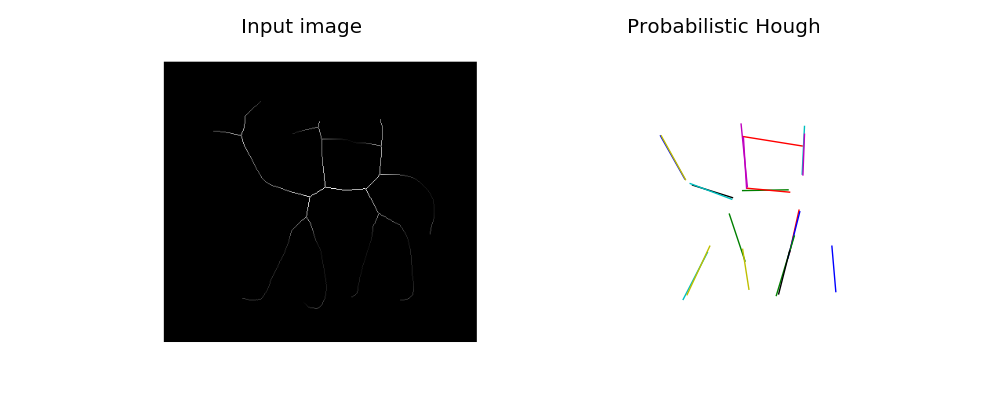
\includegraphics[scale=0.6]{camel_764.png}
\vspace{12px}

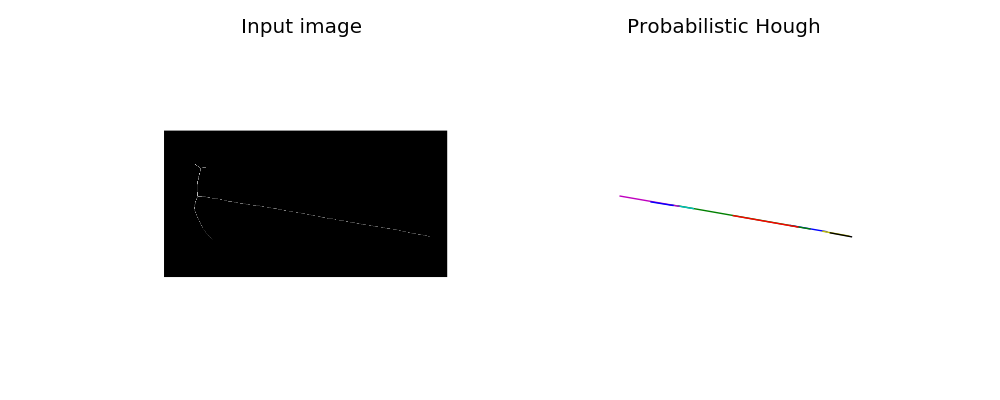
\includegraphics[scale=0.6]{hammer_604.png}

\subsubsection{Quantitive features of skeleton}
To the quantive features of the skeleton the number of branches (number of end points in skeleton)

\subsection{Border Curvature}
\subsubsection{Histogram of border curvature coefficients}

\subsection{Volumetric Features}
\subsubsection{Scaled area}
\subsubsection{Solidity and extend}
\subsubsection{Scaled major and minor axes length}
\subsubsection{Scaled centroid displacement}

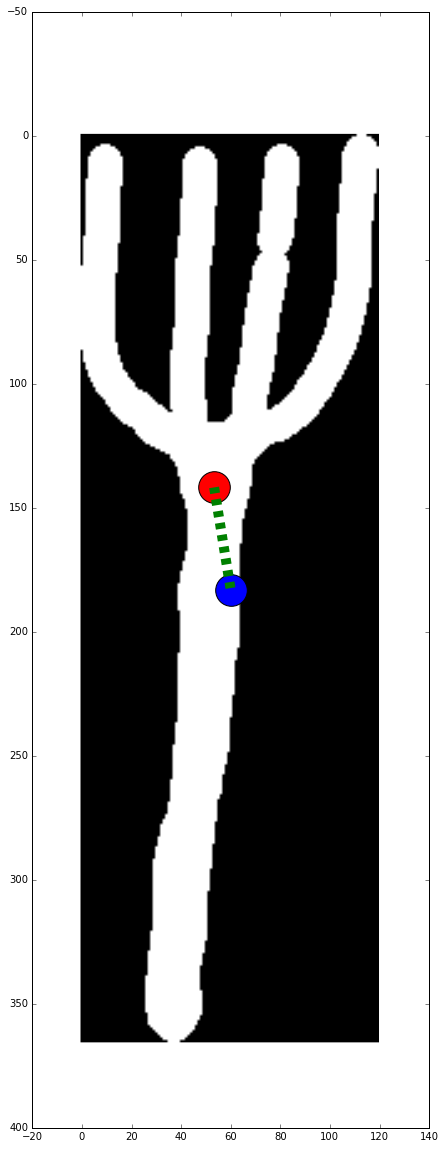
\includegraphics[scale=0.26]{fork_centroid.png}
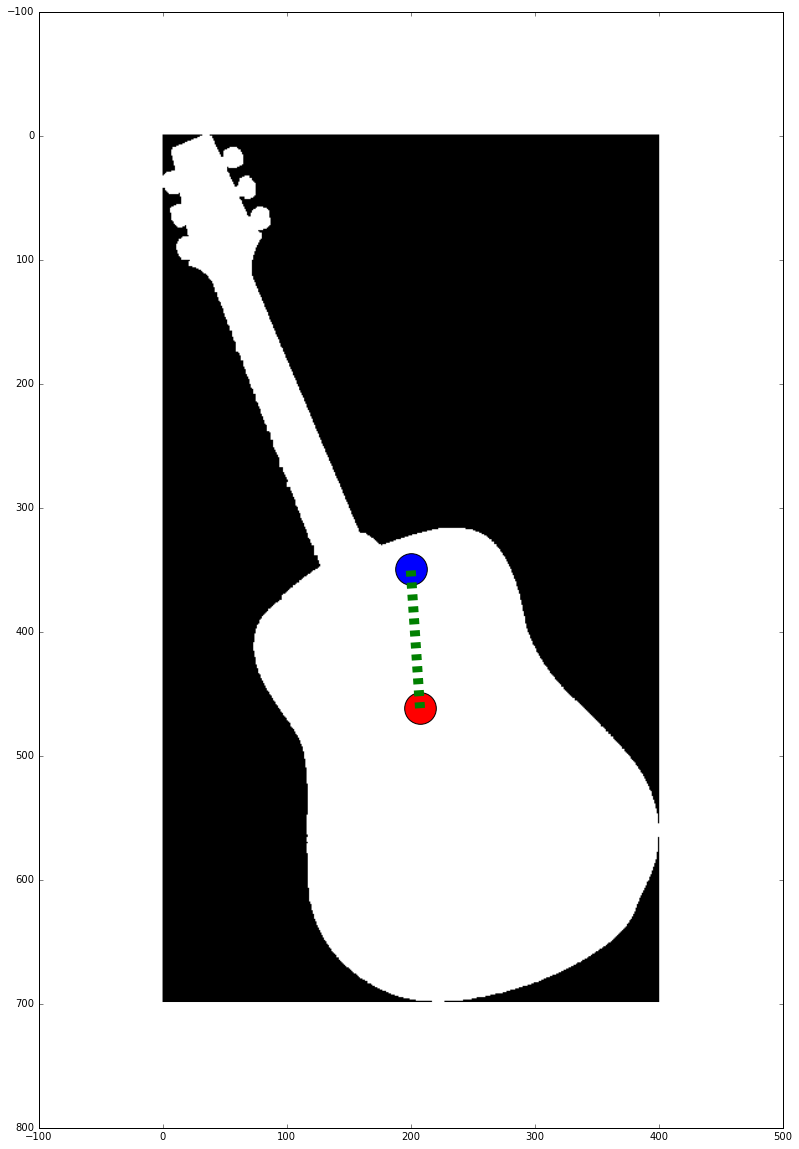
\includegraphics[scale=0.26]{guitar_centroid.png}
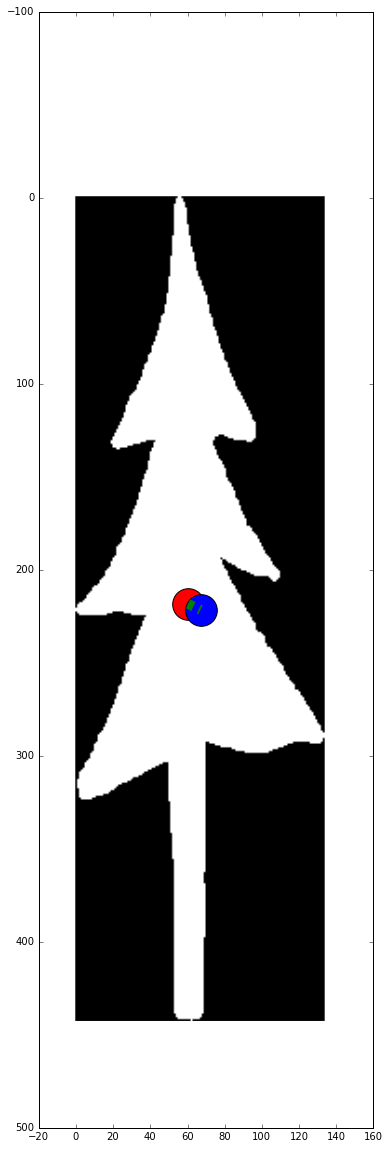
\includegraphics[scale=0.26]{tree_centroid.png}

\subsection{Assymetry measures}
Distances from original image to its horizontal and vertical flips, to rotations for $k*\frac{\pi}/4$
 
\section{Classification models}

Machine Learning techniques were used to build the model of shape recognition. 

Parameters for SVM classifiers were chosen using the grid search according to the best score.

Two kinds of test were performed on the training dataset:
\begin{itemize}
	\item \textbf{Score out of one} class which represents the accuracy score (number of samples with correctly assigned classes over all given samples).
	\item \textbf{Score out of ten} most probable classes which represents the number of samples for which the correct class was found in 10 most probable classes over all given samples.
\end{itemize}

\begin{center}
  \begin{tabular}{| l | c | c |}
    \hline
    \textbf{Classifier} & \textbf{Score out of one} & \textbf{Score out of ten}\\ \hline \hline
    \textit{Gaussian Naive Bayes} & \textit{0.79} & \textit{0.91} \\ \hline
	K-Nearest Neighbours (5 neighbours) & 0.63 & 0.87\\ \hline
	K-Nearest Neighbours (20 neighbours) & 0.5 & 0.92 \\ \hline
	SVM Classifier (linear kernel, C=1) & 0.68 & 0.90 \\ \hline
	\textit{SVM Classifier (RBF kernel, C=10, gamma=0.1)} & \textit{0.78} & \textit{0.93} \\ 
	\hline
  \end{tabular}
\end{center}


\section{Results and Discussions}
\subsection{Performance}
\subsection{Robustness and scale/rotation invariance}
\subsection{Conclusions}

\section{Bibliography}

\bibliographystyle{plain}
\bibliography{biblio}

\end{document}
